\chapter{Математичне моделювання та статистичний експеримент}
\label{chap:testing}

\section{Пошук у синтетичному сигналі}
    В цьому підрозділі розглянемо пошук шаблону в сигналі, що був згенерований як певна композиція неперервних
    функцій.

    \subsection{Пошук шаблону без модифікацій}
        Для початку порівняємо методи пошуку шаблонів використовуючи сигнал із шаблоном, котрий був доданий без
        будь"=яких видозмінень (окрім адитивного шуму/трансформації).

        В рамках експерименту на проміжку ${[0; 10]}$ із частотою дискретизації 10~КГц будувався сигнал, що складався
        з 8--16 гаусіан нормального розподілу $\dfrac{1}{\sigma\sqrt{2\pi}}
        e^{\frac{{\left(x-\mu\right)}^2}{2\sigma^2}}$
        (кількість гаусіан і їх параметри обиралися випадковим чином).
        До цього сигналу (бази) у випадкову позицію додавався шаблон виду $\sin{\alpha x^2}$.
        Приклад такого сигналу наведений на рисунку~\ref{fig:a-1}.
        На рисунку~\ref{fig:a-3} наведені відповідні ефектограми нормалізованої взаємокореляції, нормалізованої суми
        квадратів відстаней та методу на основі поліномів Кунченко.

        \todo[inline]{Вписати дані після застосування пірамідального пошуку}

        \stepcounter{tablecount}
        \begin{table}
            {|p{0.2\textwidth}|C{0.2\textwidth}|C{0.27\textwidth}|p{0.15\textwidth}|}
            {Результати пошуку шаблону без модифікації}
            {tab:a-1}

                         & Час, с & Абсолютна похибка & Екстремум\\
                \hline}
            Kunchenko & 108,01 & -0,04 & 0,06\\
            NCC       & 5,55   & -0,04 & 0,25\\
            NSSD      & 5,51   & -0,04 & 1.50\\
        \end{table}


        \stepcounter{figurecount}
        \begin{figure}[h]
            \centering
            \subfloat[Без шуму]{%
                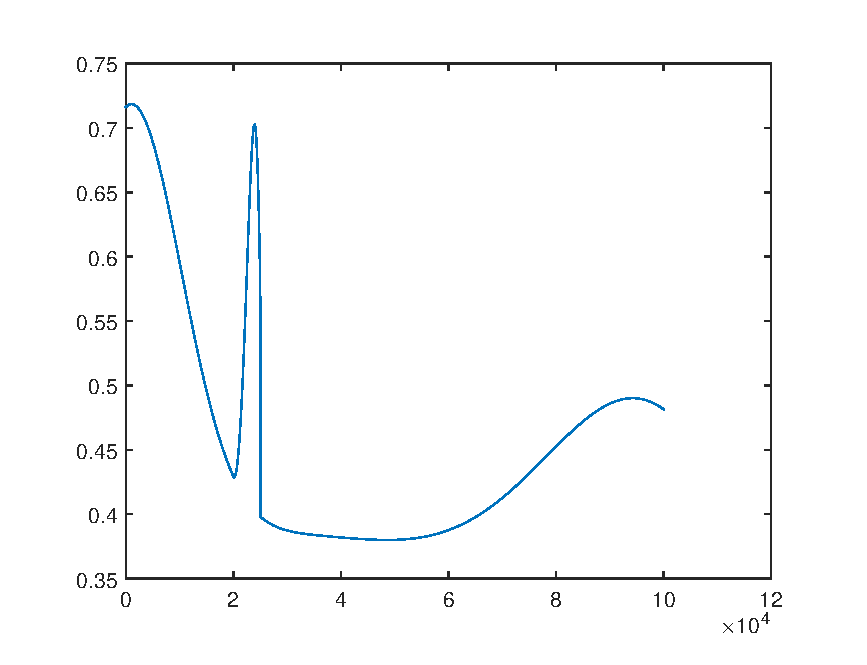
\includegraphics[width=0.8\textwidth]{a_1.eps}
            }

            \subfloat[Із шумом]{%
                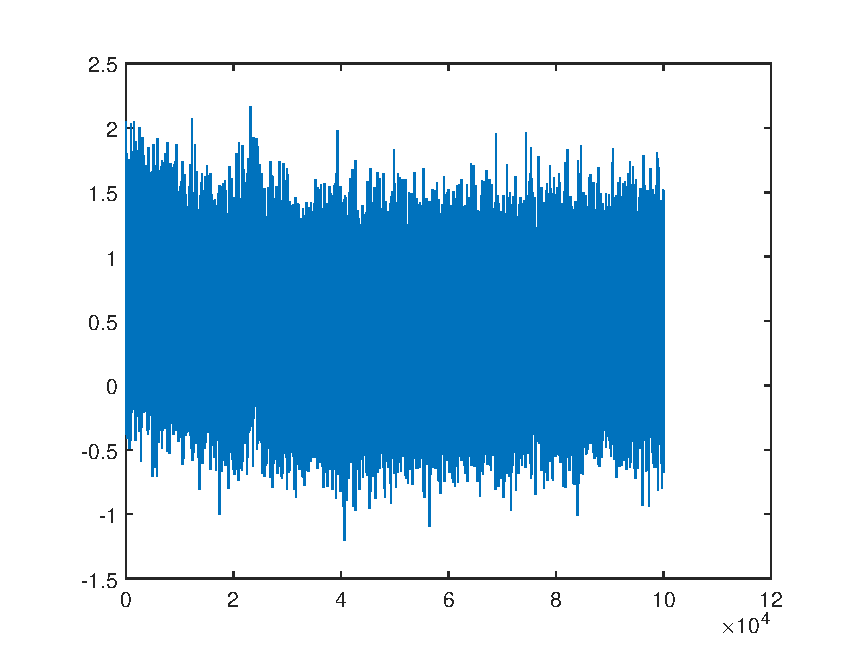
\includegraphics[width=0.8\textwidth]{a_2.eps}
            }
            \caption{Приклад сигналу із шаблоном без модифікації}\label{fig:a-1}
        \end{figure}

        \stepcounter{figurecount}
        \begin{figure}[!h]
            \centering
            \subfloat[Kunchenko]{%
                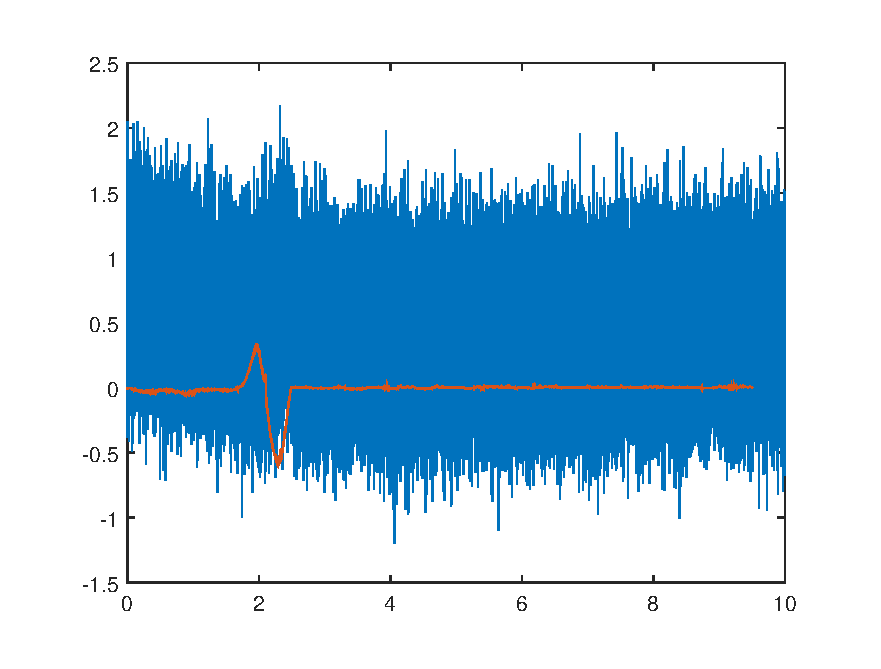
\includegraphics[height=0.28\textheight]{a_3.eps}
            }

            \subfloat[NCC]{%
                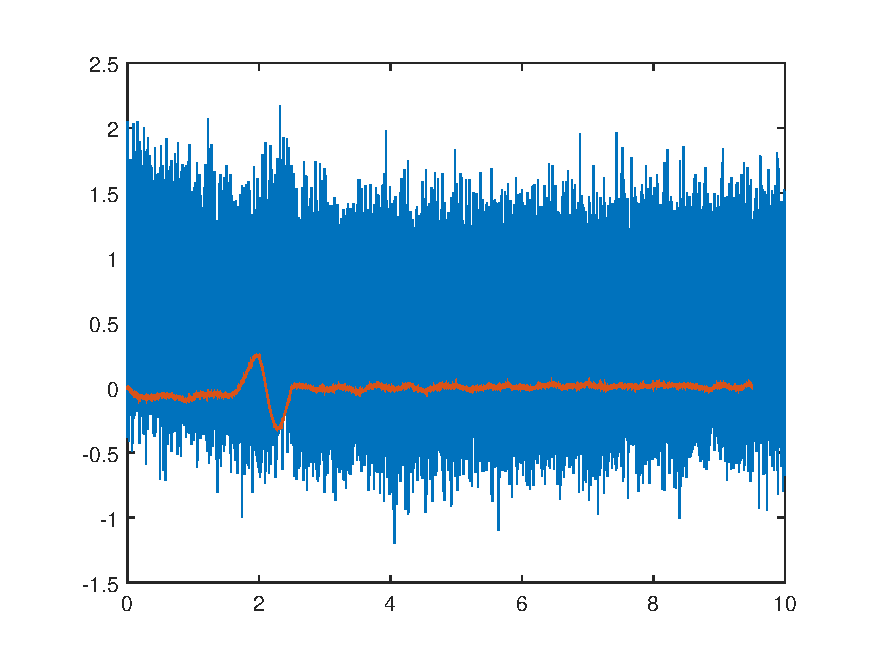
\includegraphics[height=0.28\textheight]{a_4.eps}
            }

            \subfloat[NSSD]{%
                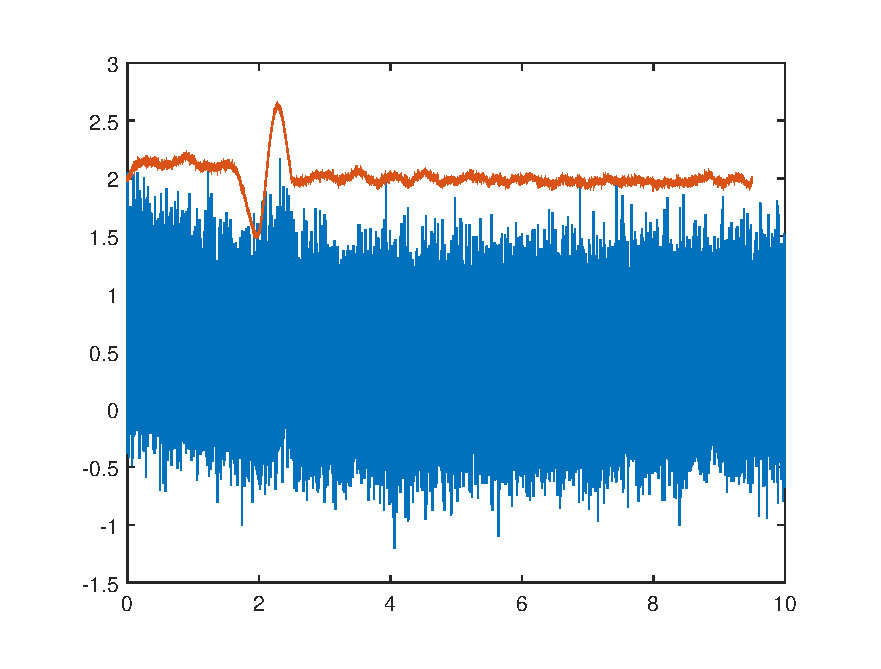
\includegraphics[height=0.28\textheight]{a_5.eps}
            }
            \caption{Пошук шаблона без модифікацій в синтетичному сигналі}\label{fig:a-3}
        \end{figure}
        У таблиці~\ref{tab:a-1} приведені дані статистичного експерименту.

    \subsection{Пошук шаблону з модифікацій}
    \todo[inline]{Привести дані статистичного експерименту №2}
\section{Пошук шаблону у мовленнєвому сигналі}
Протестуємо метод Кунченко для пошуку шаблона (аудіозапис слова) в сигналі.
\todo[inline]{Описати експеримет й його результати}
\stepcounter{figurecount}
\begin{figure}[!h]
    \centering
    \subfloat[Сигнал]{%
        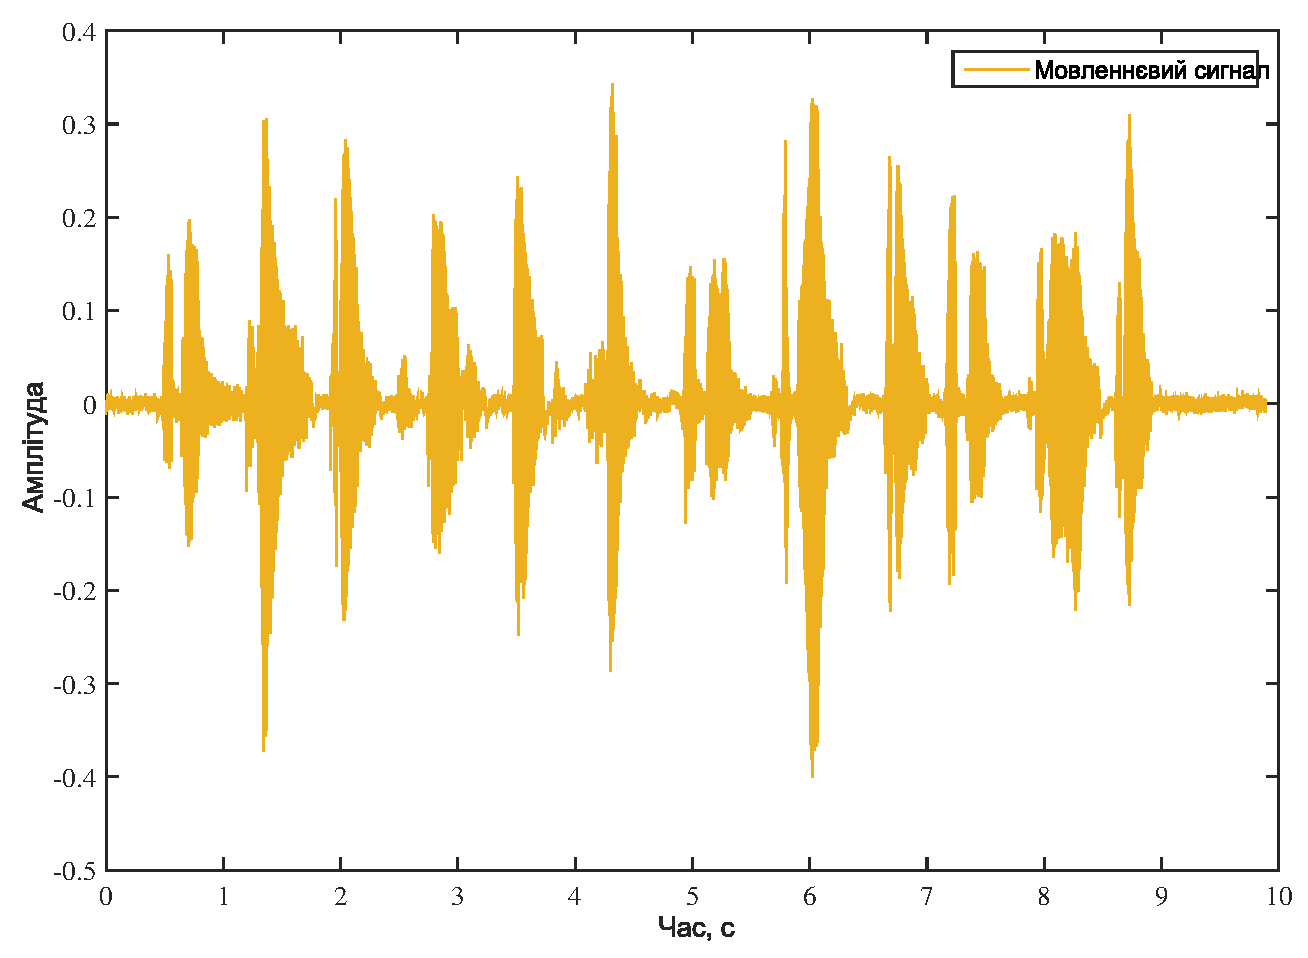
\includegraphics[width=0.8\textwidth]{audio.eps}
    }

    \subfloat[Зразок]{%
        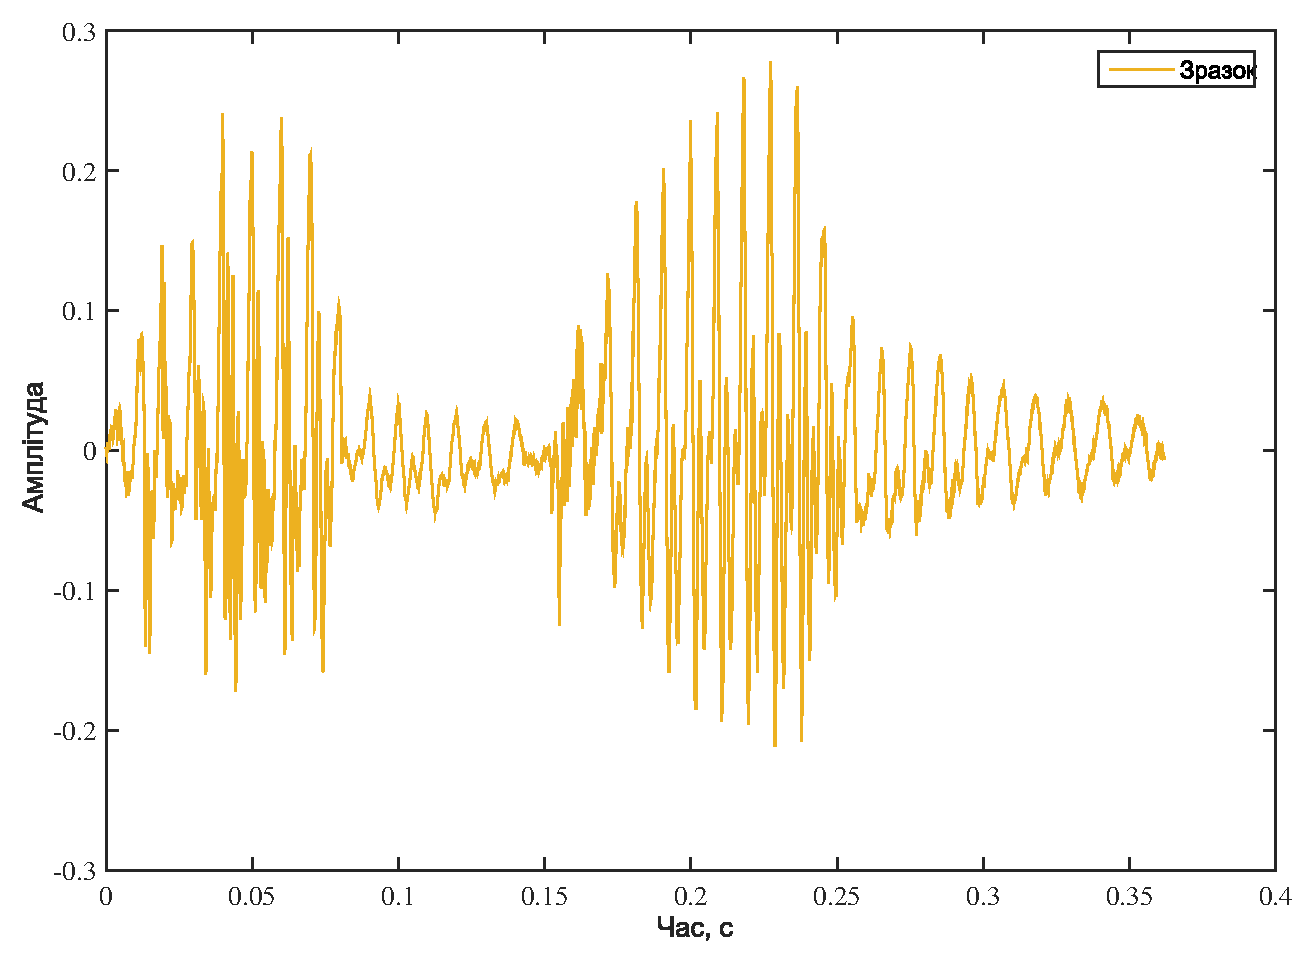
\includegraphics[width=0.8\textwidth]{audio_template.eps}
    }
    \caption{Запис мовлення й шаблон для пошуку}\label{fig:audio}
\end{figure}

\stepcounter{figurecount}
\begin{figure}[!h]
    \centering
    \subfloat[Kunchenko]{%
        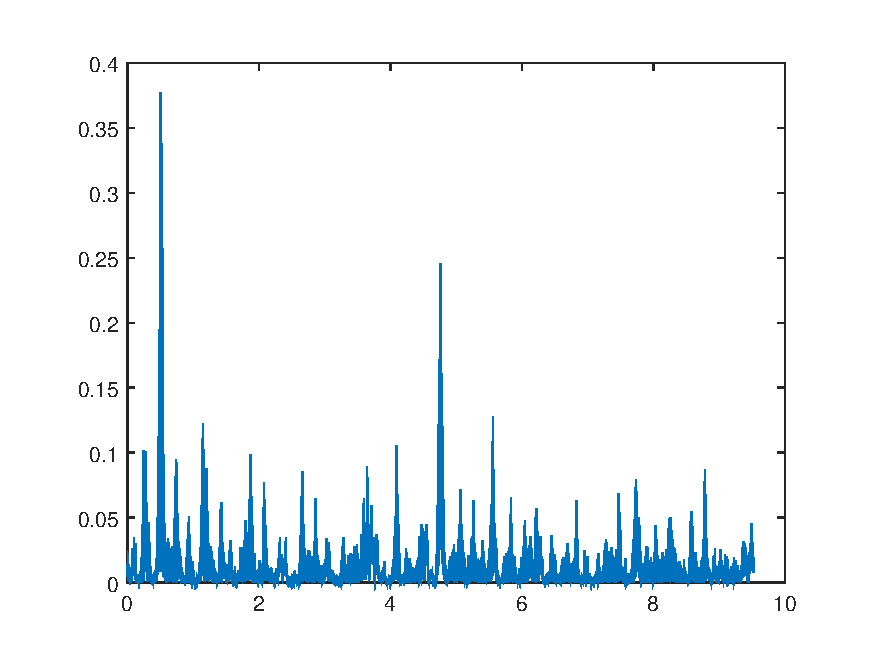
\includegraphics[height=0.28\textheight]{matched_plain_kun.eps}
    }

    \subfloat[NCC]{%
        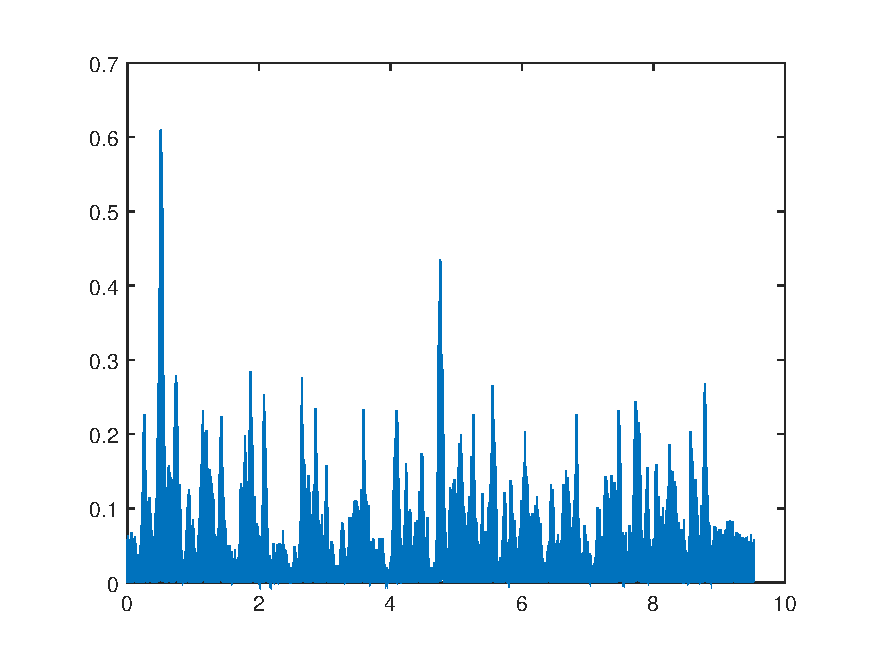
\includegraphics[height=0.28\textheight]{matched_plain_ncc.eps}
    }

    \subfloat[NSSD]{%
        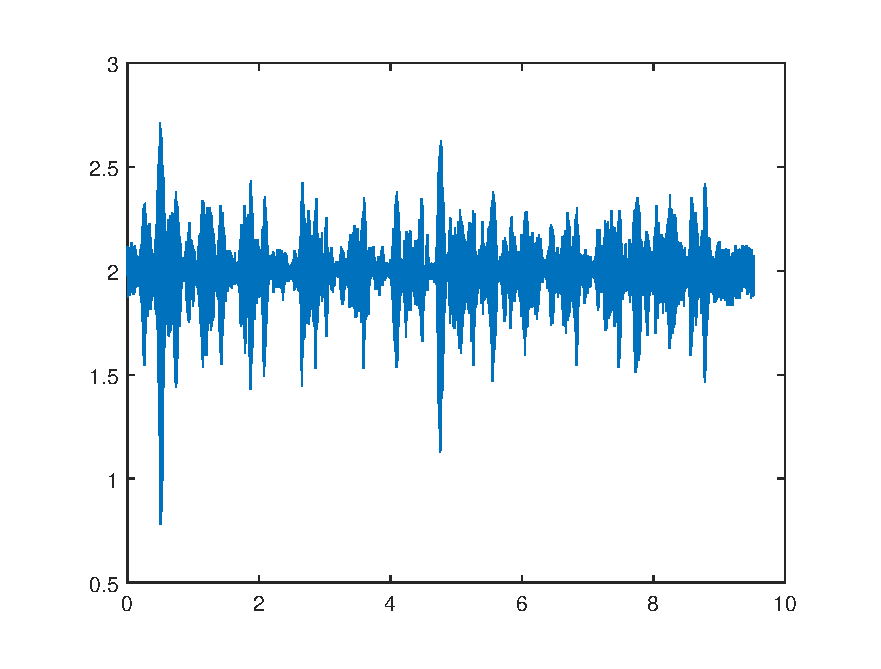
\includegraphics[height=0.28\textheight]{matched_plain_ssd.eps}
    }
    \caption{Знайдений шаблон в сигналі}\label{fig:matched-plain-audio}
\end{figure}

\stepcounter{figurecount}
\begin{figure}[!h]
    \centering
    \subfloat[Сигнал]{%
        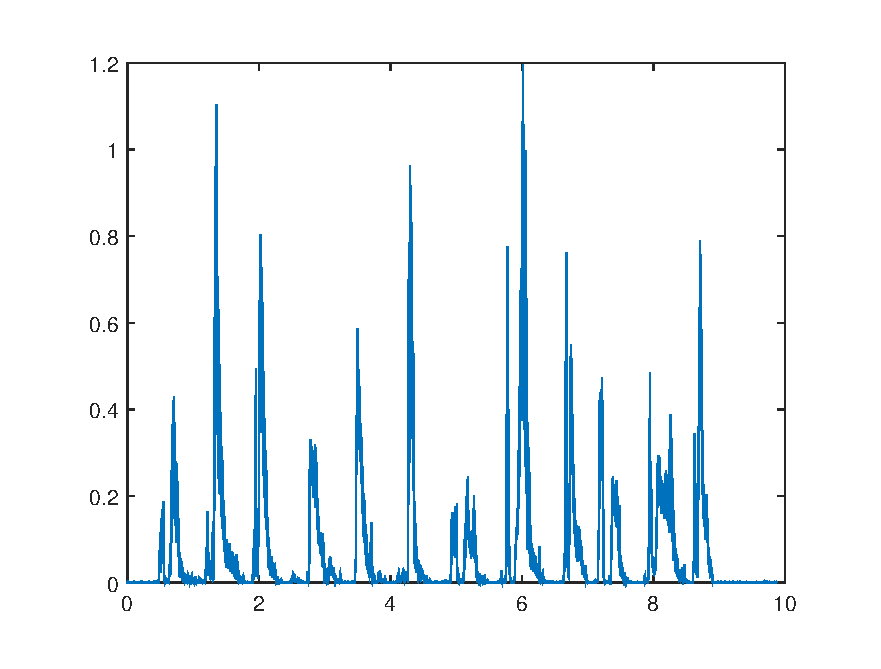
\includegraphics[width=0.8\textwidth]{audio_energy.eps}
    }

    \subfloat[Зразок]{%
        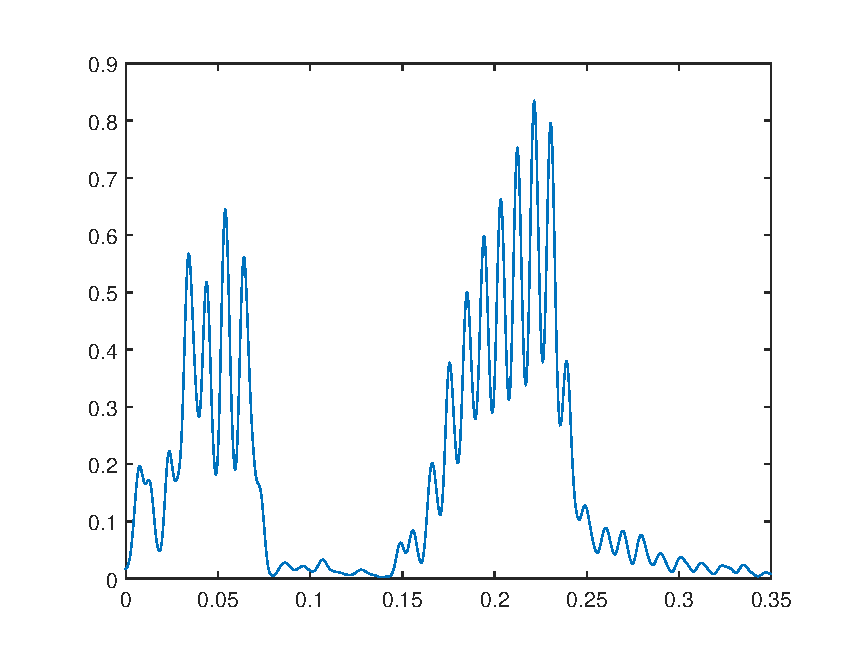
\includegraphics[width=0.8\textwidth]{audio_template_energy.eps}
    }
    \caption{Короткочасна енергія запису мовлення й шаблону для пошуку}\label{fig:audio-energy}
\end{figure}

\stepcounter{figurecount}
\begin{figure}[!h]
    \centering
    \subfloat[Kunchenko]{%
        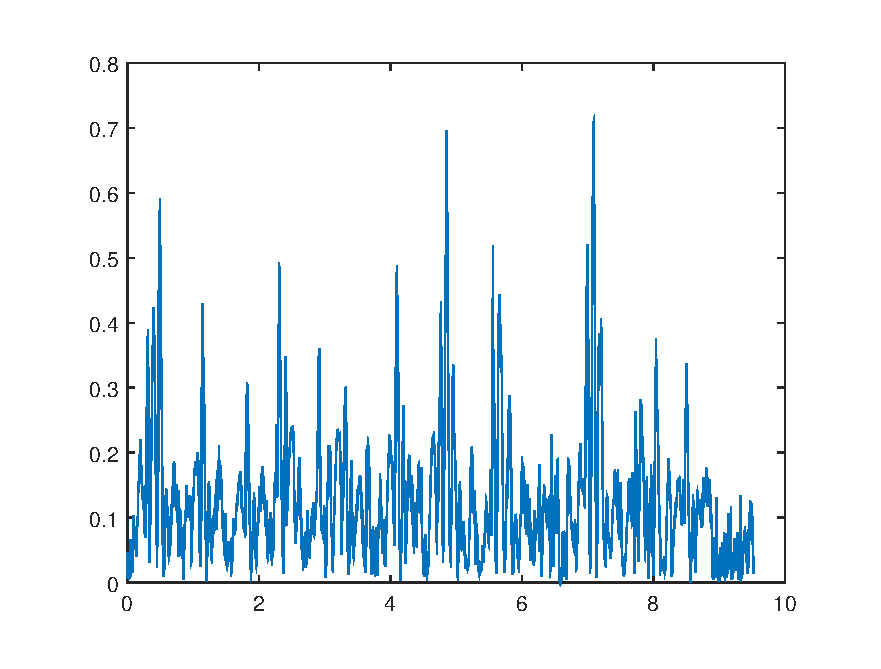
\includegraphics[height=0.28\textheight]{matched_energy_kun.eps}
    }

    \subfloat[NCC]{%
        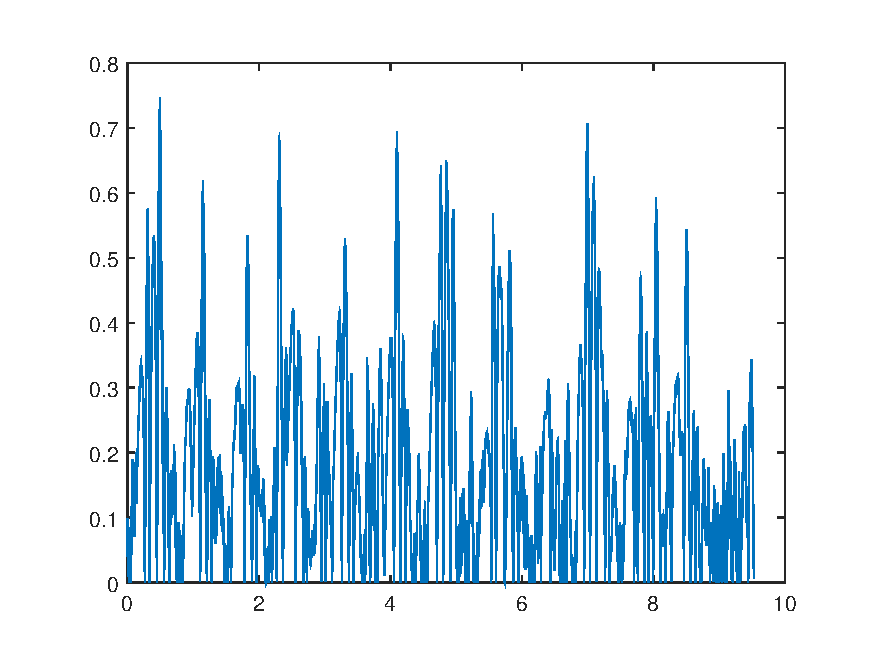
\includegraphics[height=0.28\textheight]{matched_energy_ncc.eps}
    }

    \subfloat[NSSD]{%
        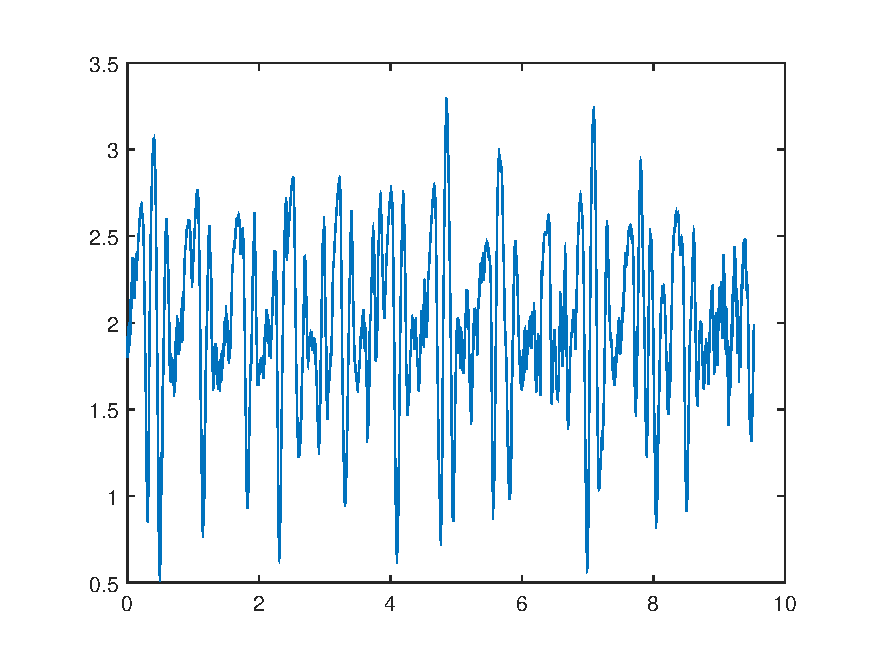
\includegraphics[height=0.28\textheight]{matched_energy_ssd.eps}
    }
    \caption{Знайдений шаблон в енергії сигналу}\label{fig:matched-energy-audio}
\end{figure}
% ncc-energy = 2.5
% ssd-energy = 2.4
% kun-energy = 86
% ncc = 2.52
% ssd = 2.85
% kun = 87



% vim: spelllang=uk,en spell filetype=tex
